\documentclass[12pt,
article,
type=prosem, %sta, diplom, bsc, pp, msc, dr, drfinal, sem, prosem
colorbacktitle,
instlogo,
accentcolor=tud1c,
twoside %TODO
]{tudthesis}

\renewcommand{\vec}[1]{\bm{#1}}

\usepackage[ngerman]{babel}
%\usepackage[english]{babel}

\usepackage[latin1]{inputenc}
\usepackage[T1]{fontenc}
%\usepackage[applemac]{inputenc}

% linebreak for urls in bitex
\usepackage{url}
\urlstyle{rm}

%listings
\usepackage{listings}
\lstset{breaklines=true, basicstyle=\small}

% clickable references
\usepackage{hyperref}

\usepackage{amsmath}
\usepackage{siunitx}

\usepackage{pgfplots} 
\pgfplotsset{compat=newest}
\usepackage{float}
\usepackage{subfigure}
\usepackage{graphicx}

\newcommand{\getmydate}{%
\iflanguage{ngerman}{%
  \ifcase\month%
    \or Januar\or Februar\or M\"arz%
    \or April\or Mai\or Juni\or Juli%
    \or August\or September\or Oktober%
    \or November\or Dezember%
  \fi\ \number\year%
}%
\iflanguage{english}{%
  \ifcase\month%
    \or January\or February\or March%
    \or April\or May\or June\or July%
    \or August\or September\or October%
    \or November\or December%
  \fi\ \number\year%
}
}
% changed counter for section wise counting
\usepackage{chngcntr}
\counterwithin{figure}{section} 
\counterwithin{table}{section} 

\setinstitutionlogo[height]{logo/ESlogo.png}

\begin{document}
	\counterwithin{lstlisting}{section}
  \thesistitle{Don't code and drive}%
    {Abschlussarbeit Projektseminar Echtzeitsysteme}
  \author{Josef Kinold, Dennis Kraus, Garwin Lechner, Blandine Riviere, Robin Scheich}
  %do not add your student id!
  %\studentidx{1145456}
	%\thesisnumber{ES-B-0060}
  \referee{Geza Kulcsar}{Geza Kulcsar}
	
  \iflanguage{english}{
		\department{	\mbox{Department of Electrical Engineering}\\ and Information Technology (FB18)\\\\Adjunct Member Department of\\ Computer Science (FB20)\\\\Prof. Dr. rer. nat. A. Sch�rr\\\ Merckstra�e 25\\64283 Darmstadt\\\\www.es.tu-darmstadt.de}
		\group{Real-Time Systems Lab}
	}{
		\department{Elektrotechnik und \\Informationstechnik (FB18)\\\\Zweitmitglied Informatik (FB20)\\\\Prof. Dr. rer. nat. A. Sch�rr\\\ Merckstra�e 25\\64283 Darmstadt\\\\www.es.tu-darmstadt.de}
		\group{Fachgebiet Echtzeitsysteme}
	}
  
  \dateofsubmit{\today}
  \makethesistitle
  %\affidavit{J. Walker}
	
	%\cleardoublepage
	%\begin {abstract}
	%...
	%\end{abstract} 

	%\cleardoublepage
	\pagenumbering{roman}
	%\addtocontents{Anhang}{}
	\tableofcontents
	%\clearpage
	%\listoffigures
	%\clearpage
	%\listoftables 
	\cleardoublepage %TODO
	
	\pagenumbering{arabic}
	\section{Einleitung}
\label{sec:einleitung}
\textbf{Im Projektseminar Echtzeitsysteme werden die Teilnehmer in Gruppen \'{a} 5 Leute aufgeteilt. Jede Gruppe bekommt ein Modellfahrzeug, welches mit Sensorik und Aktorik so ausgestattet ist, dass das Fahrzeug autonom fahren kann. Jede Gruppe sollte mit dem Fahrzeug drei Aufgabenstellungen umsetzten, wobei nur die erste, das Fahren eines Rundkurses entlang einer Wand ohne Hindernisse, vorgegeben war. Die anderen beiden Aufgabenstellungen konnte man aus einer Liste ausw\"ahlen, oder sich nach Absprache mit den Betreuern eine eigene Aufgabe ausdenken. Wir haben uns als zweite Aufgabe den Rundkurs mit Hindernissen ausgesucht, da wir gehofft haben, f\"ur die erste und zweite Aufgabenstellung denselben Ansatz verwenden zu k\"onnen. Des weiteren haben wir es uns zur Aufgabe gemacht, eine Personenverfolgung zu implementieren. Diese sollte eine Person mithilfe des Kamerabildes detektieren und ihr dann folgen, falls sie sich bewegt.}
	\clearpage
	\section{Trajektorienplanung}
\label{sec:trajektorienplanung}
Das Auto hat vorne sowie hinten jeweils zwei R\"ader, die durch einen Elektromotor ansteuerbar sind. Die Lenkung der Vorderachse ist durch einen Servomotor realisiert. Das Fahrzeug ist vorne und an den Seiten mit Ultraschallsensoren zur Abstandmessung ausgestattet und besitzt eine nach vorne ausgerichtete Kinect2 Kamera, die sowohl Farb- als auch Tiefenbild liefert. F\"ur die Bestimmung der Orientierung des Fahrzeugs sind verschiedene Sensoren verbaut. \\
Um einen Rundkurs mit oder ohne Hindernissen zu bew\"altigen, muss man die gegebenen Werkzeuge nutzen und entsprechend kombinieren um das Ziel zu erreichen. Die beiden Ans\"atzen \"uber einen PD-Abstandregler (vergleiche Abschnitt \ref{subsec:02PDregler}) und \"uber eine Trajektorienplanung (vergleiche Abschnitt \ref{subsec:02implementierung}) werden im Folgenden vorgestellt.

\subsection{Modellbildung}
\label{subsec:02modellbildung}
Um eine Beziehung zwischen physikalischer Gr\"o\ss{}e f\"ur Geschwindigkeit und Lenkwinkel und der entsprechenden Stellgr\"o\ss{}e zu herzustellen, wird jeweils ein Modell ben\"otigt.
\paragraph{Geschwindigkeitsmodell} %TODO set math envirment
Die Daten aus Abbildung \ref{fig:velocity_profile} wurden bei einer Messfahrt mit Hilfe eines rosbag aufgezeichnet und im Anschluss mit dem Tool plotjuggler ausgewertet. Dazu wurde das Fahrzeug mit Geschwindigkeitsstellgr\"o\ss{}en im Intervall von -500 bis 1000 angesteuert und die jeweilige Geschwindigkeit aus der Odometrie ausgelesen. Auff\"allig ist der Sprung am Achsenursprung, der dadurch entsteht, dass das Fahrzeug eine bestimmte Stellgr\"o\ss{}e ben\"otig, um seine Tr\"agheit zu \"uberwinden.
Die gemessenen Daten lassen sich durch eine Gerade approximieren.

%%Akku
\begin{figure}[h] %TODO replace image
\centering
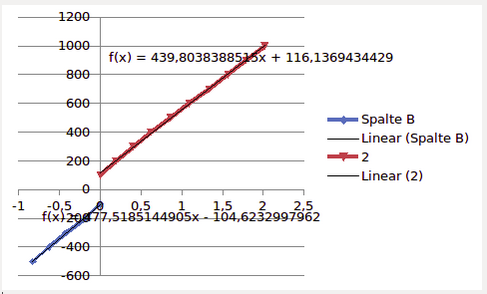
\includegraphics[width=0.7\linewidth]{pics/velocity_profile}
\caption{Geschwindigkeitsmodell}
\label{fig:velocity_profile}
\end{figure}

\paragraph{Lenkwinkelmodell}
Die Bestimmung des Lenkwinkelmodells (Abbildung \ref{fig:steering_profile}) folgte dem Schema:
\begin{itemize}
	\item Auto anheben und Stellgr\"o\ss{}e f\"ur den Lenkwinkel auf 0 setzen
	\item Mit Geschwindigkeit 300 kurz geradeaus fahren und dann Lenkwinkel einstellen
	\item Geschwindigkeit auf 0 setzen und den Lenkwinkel mit einem Geodreieck messen
\end{itemize}
Dazu war das Paket rqt\_reconfigure sehr hilfreich. Die gemessenen Daten wurden im Anschluss durch ein Polynome sechsten Grade approximiert. Auff\"alig ist die Verschiebung auf der y-Achse, die durch Offset in der Lenkung entsteht. Es sei angemerkt, dass die Messungen mit Fehlern behaftet waren und somit eine ungenaues Lenkwinkelmodell entstanden ist. Genauere Ergebnisse k\"onnte man mit Verwendung der Odometrie bei einer Fahrt im Kreis erzielen.
\begin{figure}[h] %TODO replace image
	\centering
	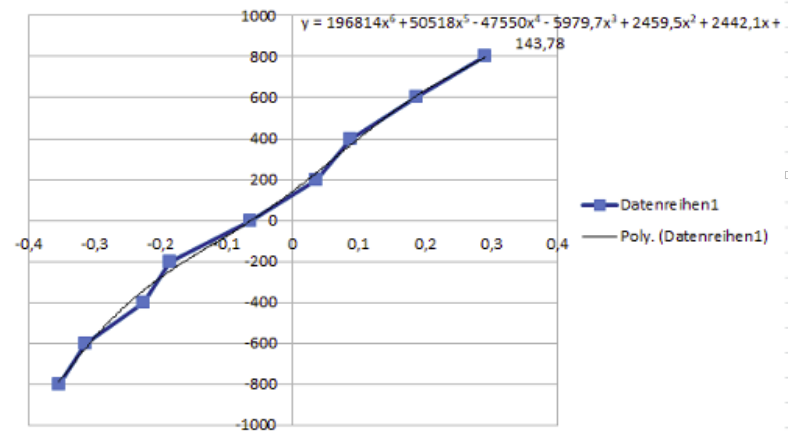
\includegraphics[width=0.7\linewidth]{pics/steering_profile}
	\caption{Lenkwinkelmodell}
	\label{fig:steering_profile}
\end{figure}
\subsection{PD Regler}
\label{subsec:02PDregler}

Ein einfacher Ansatz f\"ur den Rundkurs ohne Hindernisse ist die Abstandregelung mit Hilfe der Ultraschallsensoren und einem PID Regler. Die zu regelnde Gr\"o\ss{}e ist der Abstand zur Wand, als Stellgr\"o\ss{}e dient der Lenkwinkel. Dazu kann entweder die Stellgr\"o\ss{}e f\"ur den Lenkwinkel geregelt werden oder der Lenkwinkel selbst und dann auf die Stellgr\"o\ss{}e mit dem Lenkwinkelmodell umgerechnet werden. Die Reglerauslegung ist sowohl per Simulation in Simulink als auch experimentell durchgef\"uhrt worden. \\
Die Simulation beruht auf dem Ackermann-Modell, einem Einspurmodell f\"ur Fahrzeuge. Es lautet

\begin{align} 
	\dot{\varphi}_\text{K} &= \frac{v}{l}\cdot\tan\varphi_\text{L}\\
	\dot{y} &= v \cdot \sin \varphi_\text{K}+v\cdot\frac{l_\text{H}}{l}\cdot\cos\varphi_\text{K}\cdot\tan\varphi_\text{L}.
	\intertext{Durch Linearisierung erh\"alt man}
	\dot{\varphi}_\text{K} &= \frac{v}{l}\cdot\varphi_\text{L}\\
	\dot{y} &= v\cdot\varphi_\text{K}+v\cdot\frac{l_\text{H}}{l}\cdot\varphi_\text{L}.
\end{align}
Dabei ist $\varphi_\text{K}$ der Kurswinkel, $\varphi_\text{L}$ der Lenkwinkel, $v$ die Geschwindigkeit des Fahrzeugs, $l$ der Achsabstand, $l_\text{H}$ der Abstand von der Hinterachse zu einem Referenzpunkt und $y$ der Abstand zur Wand. Mit beiden Systemen wurde in Simulink eine PD-Reglerauslegung durchgef\"uhrt. Es wurden diskrete Systeme betrachtet (vergleiche Abbildung \ref{fig:regelkreis}), die Geschwindigkeit war $\SI[per-mode=fraction]{0.5}{\meter\per\second}$. Der simulierte Verlauf der Sprungantwort ist in Abbildung \ref{fig:SprungantwortSimulink} dargestellt, der Stellgr\"o\ss{}enverlauf in Abbildung \ref{fig:StellgroesseSimulink}.

\begin{figure}[h]
	\centering
	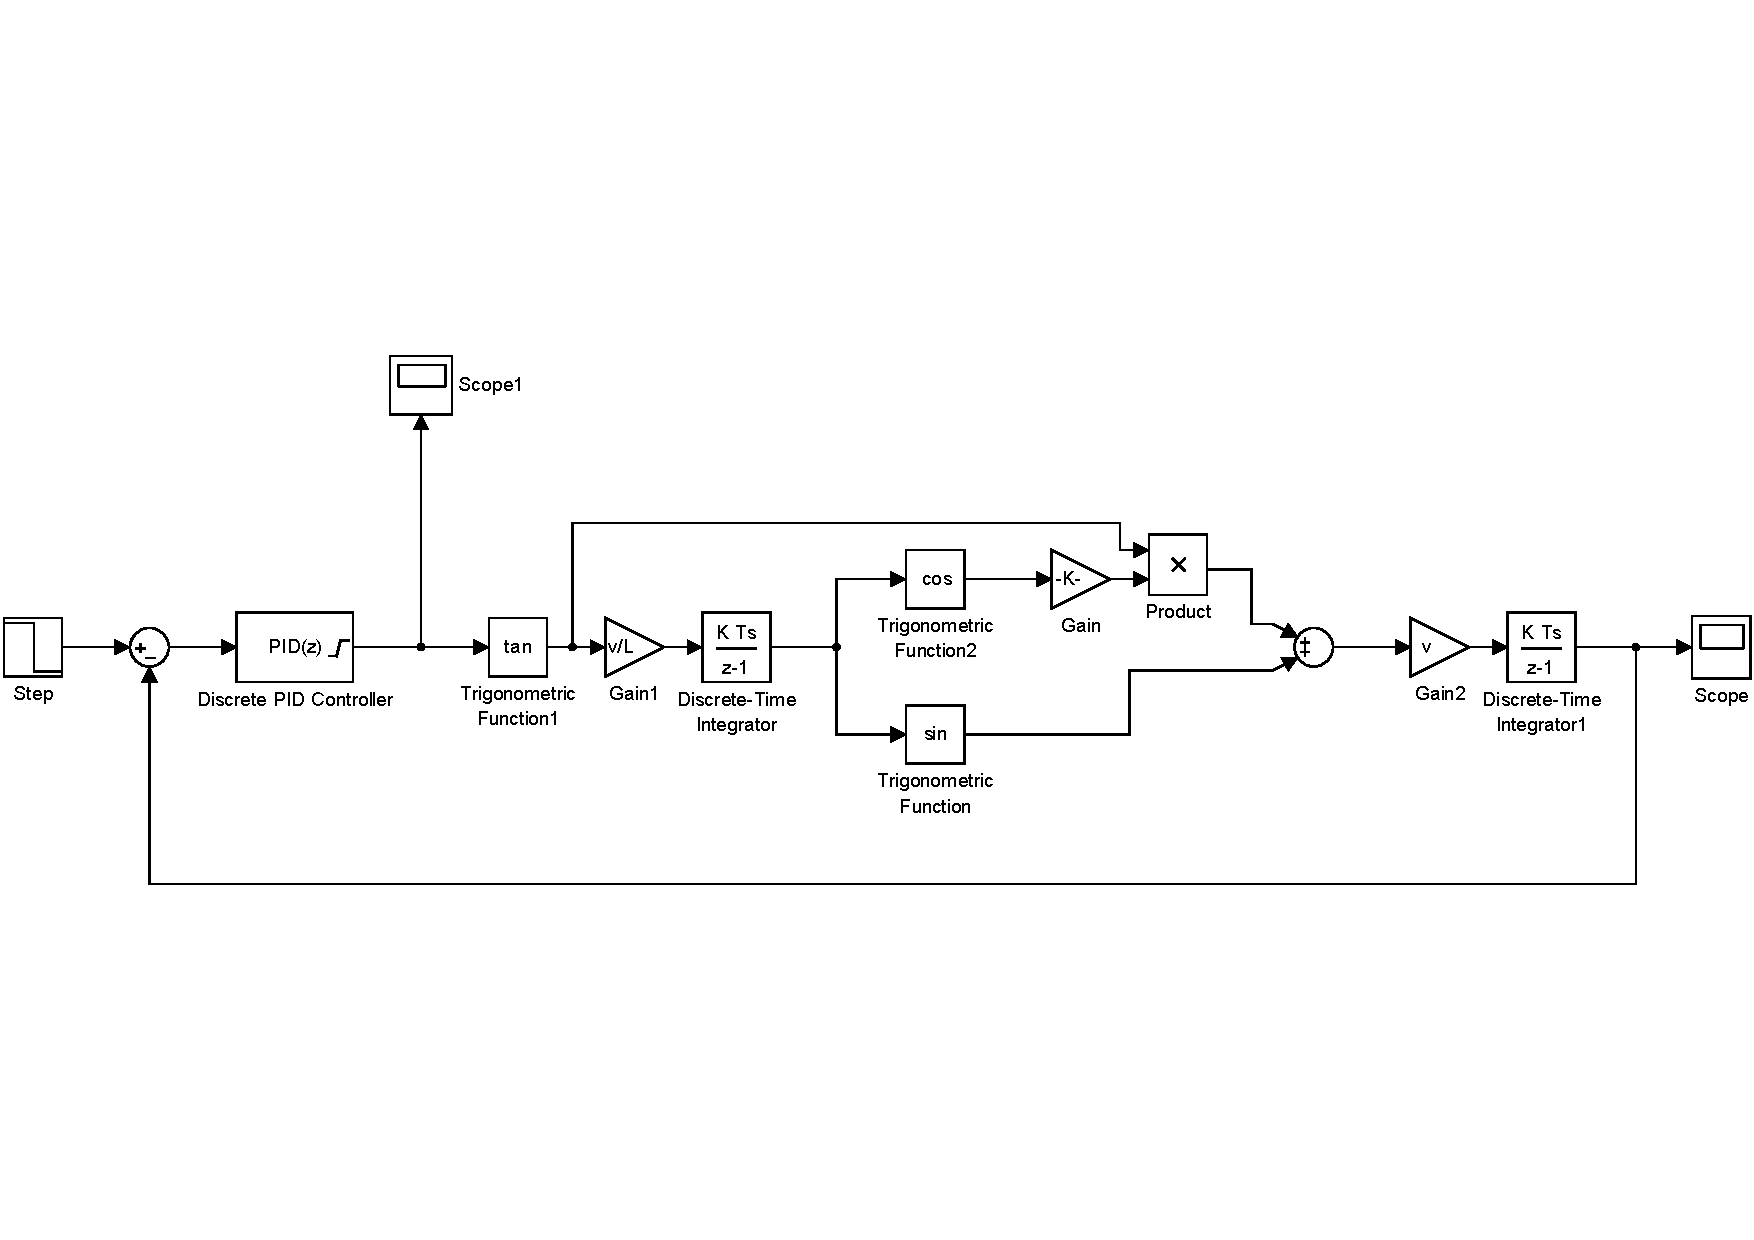
\includegraphics[width=0.9\linewidth,trim=0cm 6cm 0cm 6cm, clip]{pics/system.pdf}
	\caption{Diskreter Regelkreis mit nicht linearisieren Ackermann-Modell.}
	\label{fig:regelkreis}
\end{figure}
\begin{figure}
	\centering
	\subfigure[Sprungantwort]{
			\begin{tikzpicture}
			\begin{axis}[xlabel = Zeit in \si{\second},ylabel=Regelgr\"o\ss{}e in \si{\meter},xmin=0,xmax=9,ymin=0.2, ymax=0.9, axis x line=bottom, axis y line=left,grid,width=7cm,height=5cm]
			\addplot[mark=none,very thick] table [col sep=semicolon] {pics/sprungantwortSimulink.csv};
			\end{axis}
			\label{fig:SprungantwortSimulink}
			\end{tikzpicture}}
	\subfigure[Stellgr\"o\ss{}e]{
			\begin{tikzpicture}
			\begin{axis}[xlabel = Zeit in \si{\second},ylabel=Stellgr\"o\ss{}e in \si{\meter \per \second},xmin=0,xmax=9,ymin=-0.4, ymax=0.4, axis x line=bottom, axis y line	=left,grid,width=7cm,height=5cm]
			\addplot[mark=none,very thick] table [col sep=semicolon] {pics/stellgroesseSimulink.csv};
			\end{axis}
			\label{fig:StellgroesseSimulink}
			\end{tikzpicture}}
	\caption{Simulierte Verl\"aufe des Systems mit $K_\text{p}=10$ und $K_\text{d}=3$.}
	\label{fig:Simulink}
\end{figure}

Mit den gefundenen Parametern konnten keine guten Ergebnisse erzielt werden, der Fahrzeug hat den gew\"unschten Abstand zur Wand nicht eingehalten und ist stark geschwungen. Das ist auf die Ann\"aherung \"uber das Ackermann-Modell und den betrachteten Abstand zu Wand zur\"uckzuf\"uhren. Angenommen wird der Abstand senkrecht zur Wand, der in Wirklichkeit vom Fahrzeug gemessene ist bei schr\"agem Stand jedoch gr\"o\ss{}er. Die Parameter wurden manuell modifiziert und ein zufriedenstellendes Ergebnis erzielt (vergleiche Tabelle \ref{tab:PD}).

\begin{table}[h]
	\centering
	\begin{tabular}{rcc}
		 & $K_\text{p}$ & $K_\text{d}$ \\ 
		Simulink & 10 & 3 \\ 
		Experimentell & 0.48 & 1.5
	\end{tabular}
	\caption{Werte f\"ur PD Regler aus Simulation und experimenteller Bestimmung.}
	\label{tab:PD}
\end{table}

Da die Ergebnisse nicht zufriedenstellend und die L\"osung f\"ur den Rundkurs mit Hindernis nicht praktikabel ist, wurde dieser Ansatz verworfen und am Navigation Stack gearbeitet.

\subsection{Lokalisierung}
\label{subsec:02lokalisierung}

Die Trajektorienplanung des Roboters erfolgt anhand seiner Umgebungskarte, die mit den Sensordaten regelm"a"sig aktualisiert wird. Damit eine gute Trajektorie berechnet werden kann, muss das Fahrzeug in der Lage sein, sich zuverl"assig in der Karte zu lokalisieren. Dies erfordert unter anderem eine verl"assliche Odometrie, die im Abschnitt \ref{subsec:02odom} vorgestellt wird. Um die Position des Fahrzeugs in der Karte genauer zu sch"atzen, wird au"serdem das AMCL-Paket verwendet, wie im Abschnitt \ref{subsec:02amcl} beschrieben ist.

\subsubsection{Odometrie}
\label{subsec:02odom}
Auf dem Fahrzeug befinden sich ein Drei-Achs-Geschwindigkeitssensor und ein Drei-Achs-Gyroskop, welche etwa alle $\SI{0.5}{\milli\second}$ neue Werte zur Verf\"ugung stellen. Diese werden im vorhandenen Odometriepaket \texttt{pses\_odometrie} genutzt um eine Position und die Ausrichtung des Fahrzeugs anzugeben. Durch das Rauschen der Sensoren unterscheidet sich die tats\"achliche Position  nach einiger Zeit von der angegebenen Fahrzeugposition. Die IMU (inertial measurement unit) wird im Odometriepaket zwar zu Beginn kalibriert, dies bedeutet jedoch nur, dass ein festgelegter, im Stand gemittelter Rauschwert ber\"ucksichtigt und von den IMU Daten subtrahiert wird.\\
Die Verwendung eines Extended Kalmanfilters (EKF) erm\"oglicht die Verwendung verschiedener Sensoren als Eingangsgr\"o{\ss}en f\"ur die Sch\"atzung der Fahrzeugposition und der Ausrichtung. Der EKF berechnet aus dem aktuellen Zustand anhand eines nicht-linearen Zustands\"ubergangsmodells eine Absch\"atzung f\"ur den n\"achsten Fahrzeugzustand. Durch die Verwendung mehrerer Sensoren kann die Genauigkeit und Zuverl\"assigkeit der Sensoren mithilfe einer Gewichtung der Eingangsgr\"o{\ss}en des EKF ber\"ucksichtigt werden.  Die Zustandssch\"atzung wird mit der n\"achsten Messung verglichen und die Gewichtung der Sensoren dynamisch angepasst.\\
Wir haben uns f\"ur das \texttt{robot\_localization} Paket entschieden. Dies enth\"alt einen EKF, das es erm\"oglicht die Sensoren modular einzubinden und sensorspezifisch zu entscheiden, welche Daten weiterverarbeitet werden sollen.
Das Paket kann vier verschiedene Topic-Typen verarbeiten:
\begin{itemize}
	\item \texttt{nav\_msgs/Odometry} enh\"alt Positions- und Ausrichtungsdaten
	\item \texttt{geometry\_msgs/PoseWithCovarianceStamped} enth\"alt Positionsdaten
	\item \texttt{geometry\_msgs/TwistWithCovarianceStamped} enth\"alt Ausrichtungsdaten
	\item \texttt{sensor\_msgs/IMU} enth\"alt die Rohdaten aus der Inertialen Messeinheit (IMU)
\end{itemize}
Um die Sch\"atzung zu vereinfachen wird angenommen, dass sich das Fahrzeug nur im zweidimensionalen Raum befindet und nur in X-Richtung fortbewegen kann. Z-Koordinate, Roll- und Pitch Winkel sind daher konstant Null. Die Beschleunigung in Y-Richtung wird als Eingangsr\"o{\ss}e vernachl\"assigt. \\
Das \texttt{robot\_localization} Paket erm\"oglicht es, die Kamera in Verbindung mit \hyphenation{AMCL} AMCL, dem Hall-Sensor und der IMU als Eingangsgr\"o{\ss}en f\"ur das EKF zu verwenden. Aus Zeitgr\"unden haben wir das EKF nicht fertig eingestellt, stattdessen verwenden wir f\"ur die Lokalisierung die Odometriedaten in Verbindung mit AMCL, wie im Abschnitt \ref{subsec:02amcl} beschrieben wird. Dies liefert uns eine ausreichend genaue Fahrzeugposition und Ausrichtung.

\subsubsection{AMCL}
\label{subsec:02amcl}

Zur Lokalisierung des Autos wird das von ROS bereitgestellte AMCL-Paket verwendet. Dieses Paket implementiert den probabilistischen \emph{Adaptive Monte Carlo Localization} - Algorithmus und erm"oglicht dadurch die 2D-Lokalisierung von Robotern in einer vorgegebenen Karte. Die Daten aus dem Laserscan werden auf die Karte projiziert, woraus die wahrscheinlichsten Position und Ausrichtung des Fahrzeugs bestimmt werden.\\
Zu diesem Zweck ben"otigt es mehrere Informationen, n"amlich : 
\begin{itemize}
\item einen Laserscan, der aus den Kameradaten erzeugt wird 
\item die Transformationen zwischen den verschiedenen Koordinatensystemen des Roboters
\item die initiale Position des Roboters, die in unserem Fall manuell durch Rviz "ubergeben wird
\item die Karte, in der der Roboter sich orten soll
\end{itemize}

Diese Topics werden gleicherma"sen vom Navigation Stack ben"otigt und werden deswegen im entsprechenden Kapitel (siehe \ref{subsec:02implementierung}) n"aher beschrieben.\\
Allerdings ist darauf hinzuweisen, dass AMCL eine explizite Transformation vom Laserscan-Frame (hier, \texttt{base\_laser}) zum Odometrie-Frame (hier, \texttt{odom}) erfordert.\\
Das AMCL-Paket stellt ebenso eine ganze Menge von einstellbaren Optimierungsparametern bereit. Es ist zum Beispiel m"oglich das Odometriemodell (\texttt{omni} bzw. \texttt{diff} f"ur Roboter mit omnidirektionalem bzw. Differentialantrieb) auszuw"ahlen, sowie die entsprechenden Parametern einzustellen. Aus zeitlichen Gr"unden wurde jedoch eine im Navigation Stack bereits vorhandene Launchdatei f"ur differentialgetriebene Fahrzeuge (\texttt{amcl\_diff.launch}) verwendet.
\subsection{SLAM}
\label{subsec:02slam}

Die Abk"urzung SLAM steht f"ur \emph{Simultaneous Localization And Mapping} und besteht f"ur einen Roboter darin, gleichzeitig eine Karte seiner Umgebung zu erstellen bzw. zu verbessern und sich darin zu lokalisieren. In ROS stehen mehrere Pakete zur Verf"ugung, welche SLAM implementieren, die bekanntesten sind \texttt{gmapping} und \texttt{hector\_slam}. Letzteres hat die Eigenschaft, dass es keine Odometriedaten ben"otigt und nur anhand des Laserscans die Karte erstellt.\\
Um eine realistische Karte aufzubauen sind mehrere Aspekte zu beachten. Das Fahrzeug sollte langsam und m"oglichst geradeaus (ohne Schwingungen) fahren, um zu vermeiden, dass Fehldetektionen in die Karte eingebaut werden. Die Verwendung der vom Fachgebiet bereitgestellten Pakete \texttt{pses\_dashboard} und \texttt{CarControl-App} k\"onnen zur Steuerung des Fahrzeugs genutzt werden. Falls \texttt{gmapping} benutzt wird, h\"angt die Qualit"at der Karte und Lokalisierung ebenso von der Genauigkeit der Odometriedaten ab.\\
Das \texttt{hector\_slam}-Paket wurde zum Aufbau einer Karte des Fachgebiets verwendet. Da die Qualit"at der Karte jedoch nicht zufriedenstellend war, wurde die von den Tutoren vorgelegte Karte verwendet.
\subsection{Implementierung und Umsetzung}
\label{subsec:02implementierung}

\subsubsection{Navigation Stack}
\label{subsubsec:02navigatinStack}

\paragraph{Costmap}
\paragraph{Globaler Planer}
\paragraph{Lokaler Planer}
\paragraph{TF}
\subsubsection{psesTrajectory TODO} %TODO
\label{subsec:02psesTrajectory}
\paragraph{Modelle}

\paragraph{Zielsetzung}

\subsection{Ergebnisse und Probleme}
\label{subsec:02ergebnisse}
Wie im Kapitel \ref{subsec:02odom} bereits erw\"ahnt, wurde das Extended Kalmanfilter nicht fertig eingestellt. Das implementierte EKF benutzt die IMU-Daten und die Geschwindigkeit, welche mit Hilfe des Hall-Sensors berechnet wird. Obwohl die $y$-Geschwindigkeit des Fahrzeugs nicht als Eingabegr\"o{\ss}e f\"ur das EKF verwendet wird und nur die Steuerung der Geschwindigkeit in $x$-Richtung und des Yaw Winkels zugelassen sind, bewegt sich das Auto in den gefilterten Odometriedaten des EKF seitw\"arts. Das Einstellen der maximalen Be- und Entschleunigungswerte des Fahrzeugs hat zwar zur Verbesserung der Absch\"atzung beigetragen, das Problem der seitlichen Bewegung jedoch nicht behoben.

	\clearpage
	\section{Personenverfolgung}
\label{sec:personenverfolgung}

\subsection{Modulbeschreibung} %TODO
\label{subsec:03modulbeschreibung}

\subsubsection{Detektion}
\label{subsec:03detektion}
Als grundlegender Schritt der Personenverfolgung muss eine Person in dem Kamerabild gefunden werden. Dieser Vorgang nennt sich (Personen-)Detektion. Herk�mmliche Histogram-of-Oriented-Gradients Ans�tze liefern keine zufriedenstellende L�sung bez�glich des Fahrzeugs. Daher f�llt die Wahl auf die Nutzung eines Convolutional Neural Networks kurz CNN. Diese Netze eignen sich sehr gut zur Klassifizierung von Objekten in Bildern, da sie die Zugeh�rigkeit eines Objektes zu einer Klasse mit Wahrscheinlichkeiten ausdr�cken.

Ein typisches CNN besteht aus drei Layern. Das erste ist das Convolutional Layer. Seine Eing�nge bildet das Kamerabild gefaltet mit einem Kernel bzw. einer Faltungsmatrix. Die Werte des Kernels sind dabei auf das jeweilige Problem angepasst. Das Ergebnis davon ist eine sogenannte Feature-Map. Werden nun die Ergebnisse der Faltung mit einer Aktivierungsfunktion verkn�pft, bildet dies den Ausgang der einzelnen Neuronen des ersten Layers. Bei CNNs ist die Nutzung einer Rectified Linear Unit definiert durch $f(x) = max(0,x)$ mit $x$ als Ergebnis der Faltung �blich. Die zweite Schicht bildet das Pooling Layer. Hier findet eine Ordnungsreduktion statt, indem �berfl�ssige Informationen verworfen werden. Das geschieht beispielsweise mit einem Max-Pooling. Dabei wandert ein $2 \times 2$-Quadrat �ber den Ausgang der Neuronen des Convolutional Layers und beh�lt nur die Aktivit�t des jeweils aktivsten Neurons. Der Vorteil dieses Layers ist unter anderem eine erh�hte Berechnungsgeschwindigkeit des gesamten Netzes. Den Abschluss bildet das Fully-connected Layer. Hier werden die Eing�nge des Layers Objektklassen zugeteilt.

Als Neuronales Netz zur Bew�ltigung der urspr�nglichen Aufgabe wird das \textit{Google MobileNet SSD}\cite{mobilenet} als Caffe Framework Modell verwendet, welches bereits vortrainiert ist. Ein weiterer Vorteil dieses Netzes ist die Optimierung auf ressourcenschonende Berechnungen, allerdings auf Kosten der Genauigkeit. Dieser einhergehende Nachteil wird im vorliegenden Anwendungsfall jedoch nicht als relevant erkannt. Diese Optimierung zieht eine �nderung der gew�hnlichen Struktur eines CNNs mit sich wie in Abbildung \ref{fig:pv-neural-net} dargestellt.
\begin{figure}[btp]
	\centering
	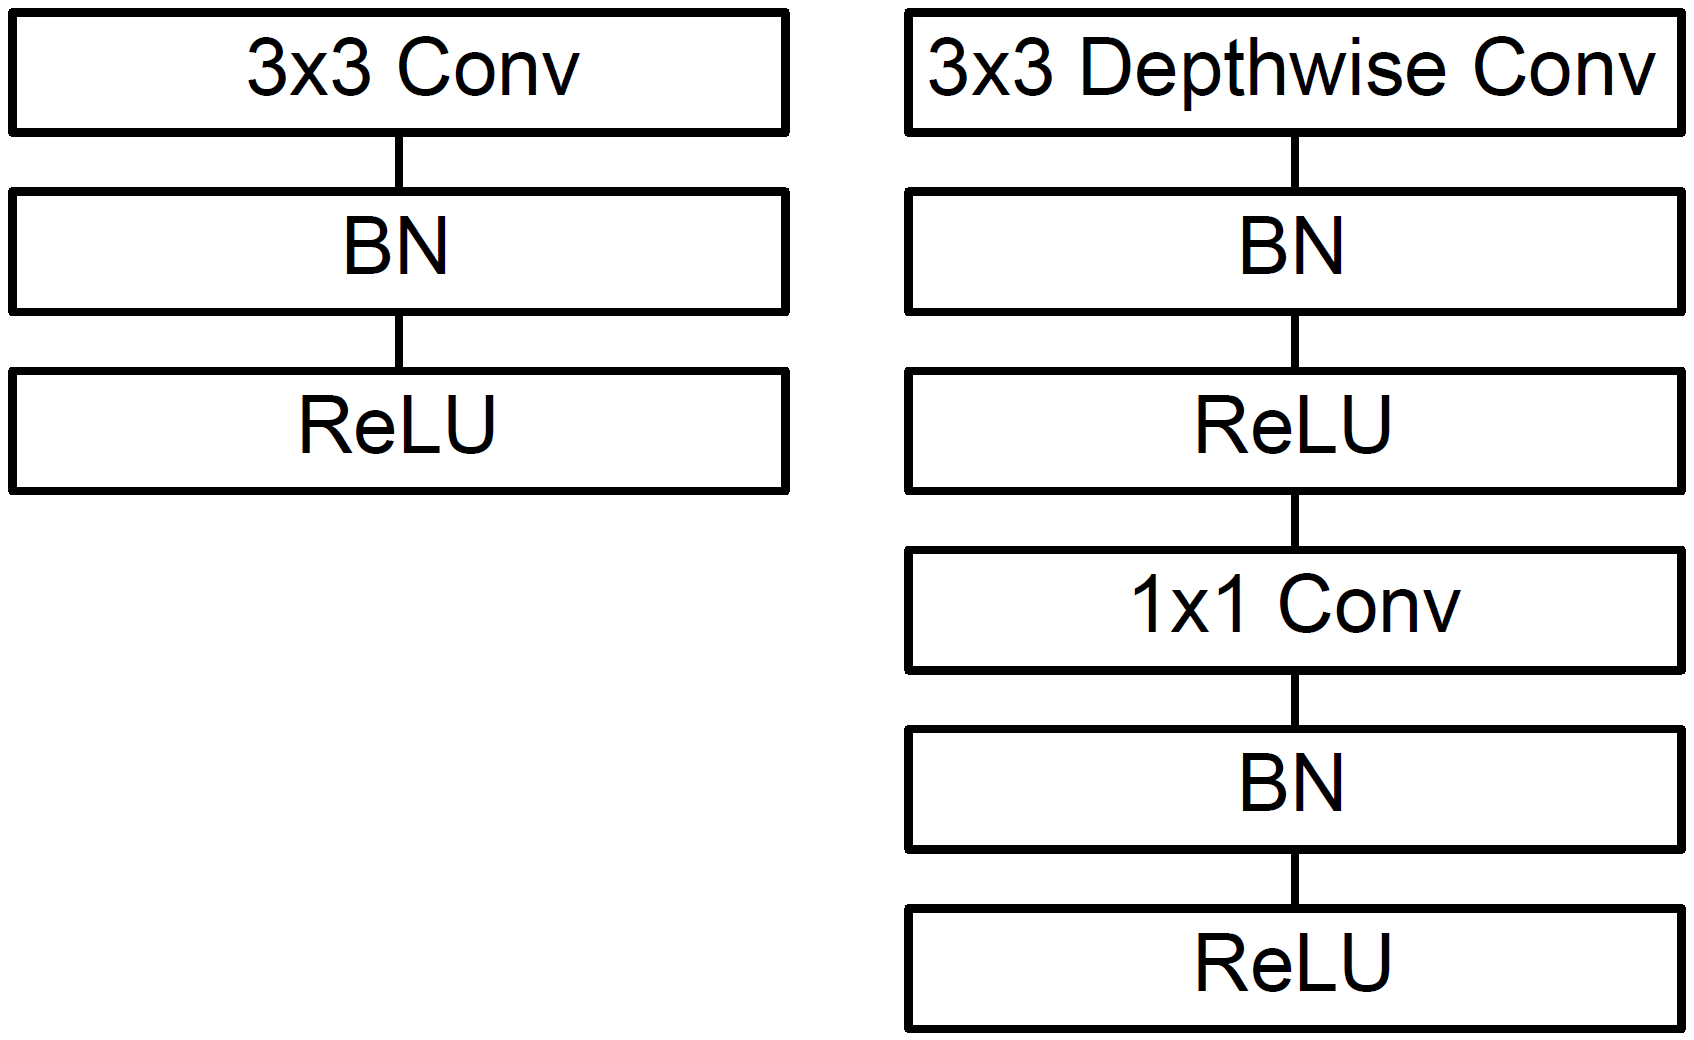
\includegraphics[width=.6\textwidth]{./pics/pv-neural-net.png}
	\caption{Links: Standard Convolutional Layer mit Batch Normalization und ReLU. Rechts: Depthwise Separable Convolutions mit Depthwise und Pointwise Layers gefolgt von Batch Normalization und ReLU. (aus \cite{mobilenet})}
	\label{fig:pv-neural-net}
\end{figure}
Die grundlegende Idee hinter Depthwise Separable Convolution ist die Aufteilung der Faltung eines CNNs in eine $3 \times 3$ Depthwise Convolution gefolgt von einer $1 \times 1$ Pointwise Convolution. Dabei dient ersteres dazu, jeden Eingangkanal zu filtern und letzteres dazu, diese Ausg�nge wieder zusammenzuf�hren. Der Vorteil davon ist die drastische Reduzierung des Berechnungsaufwands und der Modellgr��e. Batch Normalization\footnote{https://towardsdatascience.com/batch-normalization-in-neural-networks-1ac91516821c} bezeichnet dabei die Normalisierung der Werte der unsichtbaren Schichten des Netzes, um die Trainingsgeschwindigkeit deutlich zu erh�hen.

Benutzt wird das Netz mithilfe des seit OpenCV 3.3 existierenden Deep Neural Networks (dnn) Moduls. Dieses kann unter anderem Caffe Framework Modelle laden, benutzen und trainieren. Letztere Funktion wird nicht benutzt, da das Netz bereits ausreichend trainiert ist. Daher muss es lediglich einmalig zum Programmstart geladen werden. Der aktuelle Kameraframe des Farbbildes wird auf eine Gr��e von \SI{300}{px}$\times$\SI{300}{px} skaliert, da das Netz ein Eingangsbild dieser Gr��e erwartet. Anschlie�end wird der Frame vorverarbeitet. Einerseits erfolgt mit einer so genannten Mean Subtraction eine Subtraktion des Durchschnitt des jeweiligen Farbkanals vom Kameraframe, um Helligkeitsunterschieden entgegen zu wirken. Dabei wird hier der Durchschnitt auf allen Farbkan�len zu $\mu = 127,5$ gew�hlt. Andererseits kann diese Subtraktion mithilfe eines Skalierungsparameters $\sigma$ normalisiert werden. Hier wird $\sigma = 127,502231$ gew�hlt. Zu beachten ist, dass der an die \textit{blobFromImage}-Funktion �bergebende Skalierungsfaktor $1/\sigma$ entspricht. Anschlie�end kann der eben erstellte Blob dem Netz als Eingang �bergeben werden. Die Ausgabe beinhaltet alle erkannten Objekte als Matrix zusammengefasst. Eine Zeile dieser Matrix besteht aus den Eintr�gen $d^T = [0, \text{ID der zugeh�rigen Klasse}, \text{Wahrscheinlichkeit}, x, y, \text{Breite}, \text{H�he}]$. Dabei liegen die Werte der $x$- und $y$-Koordinate im Bereich $[0, 1]$ und m�ssen, um die eigentlichen Koordinaten zu erhalten, erst mit der Bildbreite bzw. Bildh�he multipliziert werden. Da unter Umst�nden mehrere Personen im Bild detektiert werden k�nnen, wird diejenige ausgew�hlt, die die gr��te Klassenwahrscheinlichkeit besitzt. Eine Alternative w�re, zus�tzlich die Wahl der Personen auf einen Bereich um den Bildmittelpunkt zu begrenzen, wenn davon ausgegangen wird, dass die zu detektierende Person frontal vor dem Fahrzeug steht. Nun ist die gew�nschte Person detektiert und es kann mithilfe der angesprochenen Koordinatentransformation eine Bounding Box der Person f�r die nachfolgenden Module erstellt werden.
\subsubsection{Tracking}
\label{subsec:03tracking}
Da die Detektion einen gewissen Rechenaufwand und somit Rechenzeit ben\"otigt, kann sie aufgrund den begrenzten Hardwareressourcen nicht regelm\"a{\ss}ig durchgef\"uhrt werden. Aus diesem Grund wird in der zweiten Phase der Personenverfolgung Tracking genutzt. \\
Tracking ist ein Vorgehen, um Objekte, in unserem Fall eine Person, in einer Folge von Bildern zu verfolgen. Der Vorteil von Tracking ist die rechensparsame Berechnung der n\"achsten Position eines Objekts, die unter gewissen Bedingungen sogar robuster als eine Detektion sein kann. Jedoch muss Tracking zu Beginn initialisiert werden, das durch die Bounding-Box der Detektion bereits gegeben ist. Zur Umsetzung des Trackings existieren verschiedene Ans\"atze, die einzelne Pixel, einen ganzen Bildteil oder Bewegungen im Bild nutzen. \\
Eine Auswahl an f\"unf Trackern wurden bereits in der OpenCV-Tracking API implementiert, sodass mehrere Tracker f\"ur die gegebene Anwendung getestet werden konnten. Die Tracker verwenden jeweils die interne Representation einer Bounding-Box und lernen abgesehen vom Median Flow einen Klassifizierer mithilfe von Online Learning\footnote{https://www.learnopencv.com/object-tracking-using-opencv-cpp-python/}. Als geeignetester Tracker stellte sich bei der Versuchsreihe der Median Flow heraus. Er bietet den besten Tradeoff zwischen Rechenzeit und Robustheit bei der Personenverfolgung. Die relativ langsamen und vorhersagbare Bewegung einer Person eignen sich gut f\"ur den gew\"ahlten Tracker. \\
Der Median Flow besteht aus zwei Hauptkomponenten. Im ersten Schritt wird die Bewegung ausgew\"ahlter Pixel mithilfe des Lucas-Kanade-Trackers berechnet und anschlie{\ss}end wird die berechnete Position durch den Forward/Backward-Error evaluiert. Die beiden Komponenten werden im Folgenden nochmal genauer beschrieben:
\paragraph{Lucas-Kanade-Tracker}
Der Lucas-Kanade-Tracker basiert auf dem Prinzip des Optischen Flusses. So kann in einer Bildfolge die neue Position eines Pixels mit folgendem Zusammenhang ausgedr\"uckt werden:
\begin{align}
I(x,y,t)=I(x+dx,y+dy,t+dt)
\end{align}
Hierbei beschreibt $I(x,y,t)$ die Intensit\"at eines Pixels an der Position $(x,y)$ zum Zeitpunkt $t$. Durch die Linearisierung mithilfe Taylorreihenentwicklung ergibt sich die Formel des Optischen Flusses zu
\begin{align}
I_{x}u+I_{y}v+I_{t} = 0 
\end{align}
mit 
\begin{align}
u=\frac{dx}{dt},\ v=\frac{dy}{dt},\ I_{x}=\frac{dI}{dx},\ I_{y}=\frac{dI}{dy},\ I_{t}=\frac{dI}{dt}.
\end{align}
Nun besteht die Aufgabe die Bewegeung $(u,v)$ zu bestimmen. Dies wird mithilfe der Erweiterung der Gleichung unter Einbeziehung der benachbarten Pixel in einem $3x3$ Fenster erm\"oglicht:
\begin{align}
\begin{pmatrix}
I_{x}(p_{1}) & I_{y}(p_{1}) \\ 
... & ...\\ 
I_{x}(p_{9}) & I_{y}(p_{9})
\end{pmatrix} 
\begin{pmatrix}
u\\ 
v
\end{pmatrix}+
\begin{pmatrix}
I_{t}(p_{1})\\ 
...\\ 
I_{t}(p_{9})
\end{pmatrix} = 0
\end{align}
Die \"uberbestimmte Formel beinhaltet die 9 Pixel $p_{1}...p_{9}$ aus dem $3x3$ Fenster und kann mithilfe der Methode der kleinsten Quadrate gel\"ost. Als Ergebnis erh\"alt man die Bewegung eines Pixels, die die Verfolgung über eine Folge von Bildern erm\"oglicht.
\paragraph{Forward/Backward Error}
Mithilfe des Lucas-Kanade-Trackers wird ein Pixels �ber eine Bilderfolge von $k$ Bildern verfolgt und so eine Trajektorie $T^{k}_{f}=(x_{t},x_{t+1},...,x_{t+k})$ bestimmt. Hierbei steht $f$ f\"ur $forward$ und beschreibt die Forw\"artstrajektorie. Das Ziel ist nun diese Trajektorie zu validieren. Hierf�r beginnen wir bei dem $x_{t+k}$ und verfolgen diesen Pixel r\"uckw\"arts �ber die gegebene Folge von $k$ Bildern. So wird eine zweite Trajektorie $T^{k}_{b}=(\hat{x}_{t},\hat{x}_{t+1},...,\hat{x}_{t+k})$ bestimmt, die mit der ersten verglichen wird. Um die Berechnung simpel zu halten, wird die euklidische Distanz zwischen Start und Endpunkt der jeweiligen Trajektorie gew�hlt:
\begin{align}
distance(T^{k}_{f},T^{k}_{b})= \left \| x_{t} - \hat{x}_{t} \right \|
\end{align} 
In Abbildung \ref{fig:ForBackError} wird das Vorgehen zur Bestimmung des Forward/Backward Errors nochmals veranschaulicht. \\
\begin{figure}[h]
	\centering
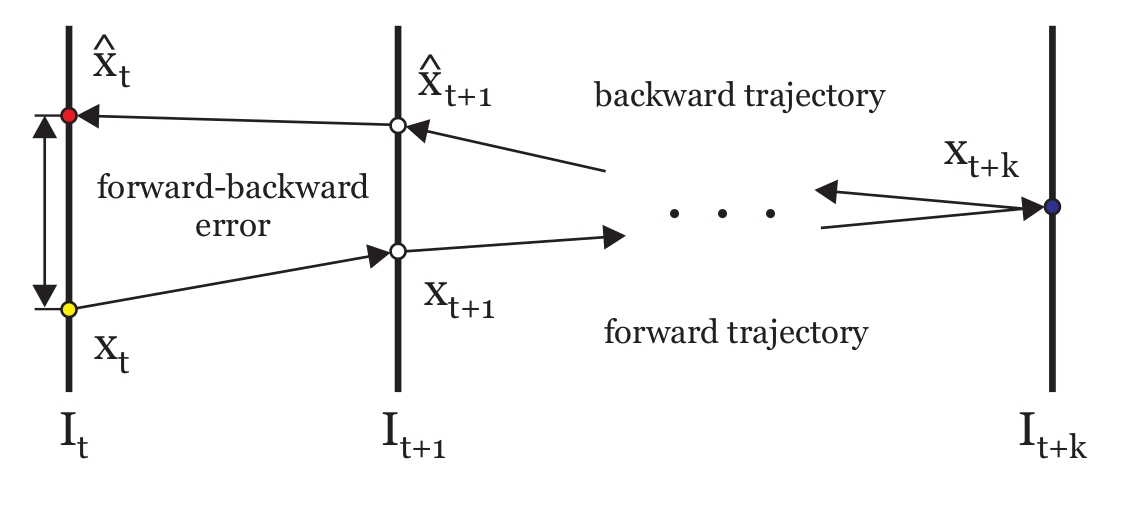
\includegraphics[width=0.6\textwidth,trim=2.4cm 0cm 0cm 1cm,clip]{pics/ForwardBackwardE.jpg}
	\caption{Das Vorgehen zur Berechnung des Forward/Backward Errors. (Quelle)}
	\label{fig:ForBackError}
\end{figure} \\

Die beschriebene Methode zur Validierung wird in der Implementierung des Median Flow zwei mal angewendet. Zu Beginn wird sie zur Auswahl der Featurpunkte aus dem Detektionfenster, die mit dem Ansatz von Lucas und Kanade getrackt werden, genutzt. So werden die Pixel, die einen hohen Forward/Backward Error aufweisen, verworfen und die signifikanten f�r Tracking geeignete Feature behalten. Weiterhin wird der Fehler zur Validierung des gesamten Trackingergebnisses genutzt und kann so ein fehlerhaftes Tracking erkennen und abrechen.
\subsubsection{Clustering}
\label{subsec:03clustering}
\subsection{Implementierung und Umsetzung}
\label{subsec:03implementierung}
Die Struktur des Algorithmus der Personenverfolgung mit ihren jeweiligen Modulen ist in Abbildung \ref{fig:personenverfolgung-struktur} dargestellt.
Dabei ist anhand der Pfeilrichtungen gut zu erkennen, wie die einzelnen Module miteinander verkn�pft sind. Anfangs wird mittels der Detektion eine Person im Farbbild detektiert und als Zielperson f�r die Anfahrt festgelegt. Letzteres wird durch die Erstellung einer Bounding Box um die Person erreicht. Da diese Detektion ziemlich rechenaufw�ndig ist, w�rde die Bildrate der Kamera bei stetiger Detektion stark abfallen. Daher ist die Kombination mit einem Tracker notwendig. Dieser wird aktiviert, sobald eine Personendetektion erfolgt und bekommt die entsprechende Bounding Box �bergeben. Da Trackeralgorithmen grunds�tzlich mit einem gewissen Drift der Position der Person bzw. des Objektes einhergehen ist eine Umschaltung zur Detektion nach einer gewissen Zeit sinnvoll, um die Korrektheit der Bounding Box wiederherzustellen. Somit findet ein stetiger Wechsel beider Module statt. Im Modul Clustering erfolgt die Berechnung der Personenkoordinaten. Dazu geschieht eine Projektion der Bounding Box vom Farbbild in das Tiefenbild. Innerhalb der projizierten Bounding Box wird die Person von der Umgebung extrahiert und ihre Tiefe bestimmt. Mithilfe dieser und der Projektionsmatrix erfolgt die Berechnung der Koordinaten der Person. Diese bekommt der Regler �bergeben, welcher daraus das finale Ziel berechnet und einen entsprechenden Lenkwinkel $\theta$ und eine entsprechende Geschwindigkeit $v$ vorgibt.
\begin{figure}[h]
	\centering
	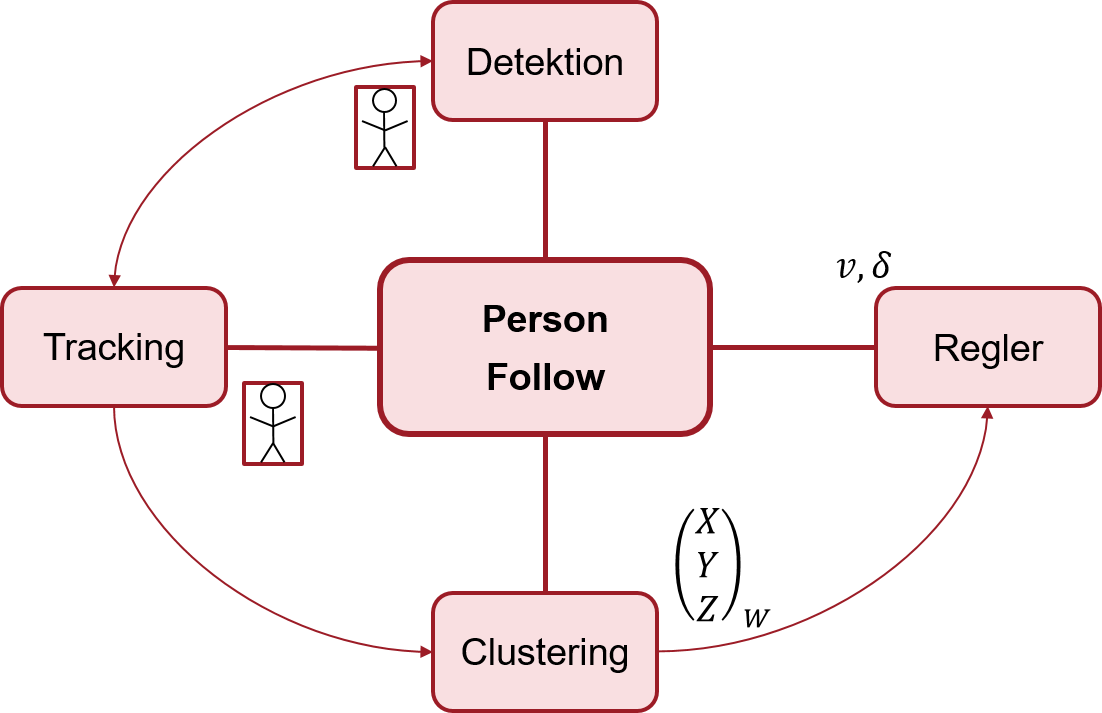
\includegraphics[width=.65\textwidth]{./pics/personenverfolgung_output.png}
	\caption{Struktur der Personenverfolgung mit jeweiligen Modulen.}
	\label{fig:personenverfolgung-struktur}
\end{figure}
\subsection{Ergebnisse und Probleme}
\label{subsec:03ergebnisse}
Die erste Versuchsreihe wird mit dem Fahrzeug auf dem Tisch platziert durchgef�hrt. Hierbei soll ausschlie�lich die Personendetektion und das Tracking ohne Bewegung des Fahrzeugs getestet werden. Die Resultat sind durchaus vielversprechend. Die Personverfolgung aus Detektion und Tracking k�nnen die Person in diesen Versuchen verl�sslich verfolgen, wobei auch fehlerhaftes Tracking erkannt wurde. Das Erkennen des misslungenen Trackings ist hingegen nicht besonders robust und somit noch ausbauf�hig. \\
In der zweiten Versuchsreihe wird die vollst�ndige Personenverfolgung samt Folgeregelung getestet. Um �berhaupt eine Person im Kamerabild zu erhalten, muss hierf�r die Kamera stark nach oben geneigt werden. Diese ver�nderte Perspektive stellt sich als Problem f�r die Personenverfolgung dar, da das Bild nun stark verzerrt wird. Sowohl die Detektion als auch das Tracking verschlechtert sich aus dieser Perspektive und sind deutlich weniger robust. Dennoch gelingt das Folgen einer Person regelm��ig f�r eine l�ngere Zeitdauer. Um die Ergebnisse in Zukunft deutlich zu verbessern, sollte eine perspektivische Transformation des Kamerabildes vor der Personenverfolgung durchgef�hrt werden. \\
Ein weiteres Problem ist die Verfolgung einer Personen um enge Ecken, da der fest eingestellte Abstand von zwei Metern f�r diesen Fall zu gro� ist. Hierf�r w�ren zwei L�sungsans�tze m�glich. Einerseits k�nnte der Abstand variabel gestaltet werden, sodass dieser bei der Fahrt um eine Ecke verringert wird. Dabei entsteht das Problem, dass die Person nicht mehr komplett im Kamerabild erfasst werden kann. Somit w�re die optimale L�sung, die Verwendung eines Kalman Filters, der die Person mithilfe der zuvor berechneten Bewegung auch au�erhalb des Kamerasichtfeldes weiter verfolgen kann. Dieses k�nnte in Kombination zum bereits implementierten Tracker eingesetzt werden und somit die gesamte Personenverfolgung verbessern.


	\clearpage
	\section{Fazit und Ausblick}
\label{sec:fazit}
	\cleardoublepage
  
	\bibliographystyle{abbrvdin}
	\bibliography{literature}
	\nocite{*}
	\cleardoublepage
	\begin{appendix}
		\section{Anhang}
\label{sec:appendix}
\subsection{Launch und Config Dateien des Navigation Stack}
\label{subsec:appendixNS}
\lstinputlisting[caption={launch/kai\_configuration.launch}]{code/launch/kai_configuration.launch}
\lstinputlisting[caption={launch/move\_base.launch}]{code/launch/move_base.launch}
\lstinputlisting[caption={cfg/base\_global\_planner\_params.yaml}]{code/cfg/base_global_planner_params.yaml}
\lstinputlisting[caption={cfg/base\_local\_planner\_params.yaml}]{code/cfg/base_local_planner_params.yaml}
\lstinputlisting[caption={cfg/costmap\_common\_params.yaml}]{code/cfg/costmap_common_params.yaml}
\lstinputlisting[caption={cfg/global\_costmap\_params.yaml}]{code/cfg/global_costmap_params.yaml}
\lstinputlisting[caption={cfg/local\_common\_params.yaml}]{code/cfg/local_costmap_params.yaml}
	\end{appendix}

\end{document}
